\section{Mel‑Scale \& Filterbanks}
\begin{frame}{}
    \LARGE \textbf{Mel‑Scale \& Filterbanks}
\end{frame}


\begin{frame}[allowframebreaks]{Mel‑Scale \& Filterbanks: Details}
    \textbf{Mel-Scale:}
    \begin{itemize}
        \item The Mel scale is a perceptual scale that reflects how humans perceive pitch differences.
        \item It maps actual frequency (Hz) to Mel frequency, aligning more closely with human auditory perception.
        \item Equal distances on the Mel scale correspond to perceived equal pitch differences.
    \end{itemize}

    \vspace{0.5em}
    The transformation from frequency $f$ (in Hz) to Mel scale $m$ is:
    \begin{equation}
        m = 2595 \cdot \log_{10}\left(1 + \frac{f}{700}\right)
    \end{equation}

\framebreak
    \textbf{Mel Filterbanks:} 
    \begin{itemize}
        \item The frequency axis is warped to the Mel scale.
        \item Typically, $N$ triangular filters (e.g., $N=40$) are created, spaced evenly in the Mel domain.
        \item Each filter collects energy from a range of frequencies, emphasizing perceptually important bands.
        \item The output is a set of Mel filterbank energies, which are used as features for audio and speech processing tasks.
    \end{itemize}

    \begin{figure}
        \centering
        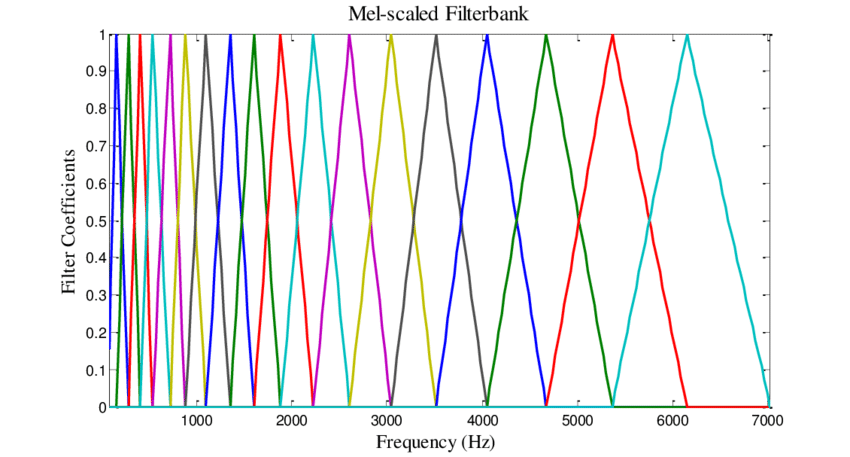
\includegraphics[width=\textwidth,height=0.8\textheight,keepaspectratio]{images/audio-nlp/mel-scaled-filterbanks.png}
    \end{figure}

\framebreak
    \textbf{Filterbank Construction Steps:}
    \begin{enumerate}
        \item Convert the lower and upper frequency bounds to Mel scale.
        \item Linearly space $N+2$ points between these bounds in Mel scale.
        \item Convert these points back to Hz to get filter edges.
        \item For each filter $k$, define a triangular response:
        \begin{equation}
            H_k(f) = 
            \begin{cases}
                0, & f < f_{k-1} \\
                \frac{f - f_{k-1}}{f_k - f_{k-1}}, & f_{k-1} \leq f < f_k \\
                \frac{f_{k+1} - f}{f_{k+1} - f_k}, & f_k \leq f < f_{k+1} \\
                0, & f \geq f_{k+1}
            \end{cases}
        \end{equation}
        \item Multiply the power spectrum by each filter and sum to get filterbank energies.
    \end{enumerate}
\end{frame}